% M. S. Tsoeu (2011), University of Cape Town <mohohlo.tsoeu@uct.ac.za>

% This is a project report templace document created for EEE4022FS students at the University of Cape Town.
%
% This file should be is processed with ``pdflatex`` and might need a few modifications if a different processor is chosen.


\documentclass[a4paper,12pt]{report}

%Include packages you need to use here

\usepackage[top = 1in, bottom = 1in, left = 1in, right = 1in]{geometry}
\usepackage{graphicx}
\usepackage{fancyhdr}
\usepackage{amsmath, amsthm, amssymb}
\usepackage{lastpage}
\usepackage{subfigure}
\usepackage{lscape}
\usepackage{hyphenat}
\usepackage{setspace}
\usepackage{hyperref}

% Include page formatting here. 
\parskip = 6mm
\parindent = 0mm
\renewcommand{\headrulewidth}{0pt}
\rhead[]{\thesection}
\lhead[\thechapter]{}


\begin{document}
 
% This section formats the title page of the Report.
\thispagestyle{empty}
{\Huge \begin{center}
% Modify the line below to insert your title.
Insert your title here
\hrule 
% Modify the line below to insert your subtitle.
{\Large Insert a subtitle here (if applicable)}
\end{center}}

\vskip 5mm
\begin{center}
\- \- \- \- \- \- \- \- \- \-
\includegraphics[scale = 0.3]{uctLogo.png}
\end{center}

\vskip 5mm
\begin{center}
Presented by:\\
Mohohlo Samuel T\v soeu		% Insert your name here
\end{center}

\vskip 10mm
\begin{center}
Prepared for:\\
M. S. T\v soeu\\ 		% Insert your supervisor's name here.
Dept. of Electrical and Electronics Engineering\\University of Cape Town
\end{center}


\vskip 10mm
\begin{center}
Submitted to the Department of Electrical Engineering at the University of Cape Town in partial
fulfilment of the academic requirements for a Bachelor of Science degree in ***INSERT DEGREE
NAME HERE (Electrical Engineering; Mechatronics or Electrical and Computer Engineering)

\end{center}


\vskip 5mm
\begin{center}{\bf \today}
\end{center}

\newpage
\thispagestyle{empty}
\mbox{}
\newpage

\onehalfspacing
\nohyphens{
\thispagestyle{empty}
\vskip 40mm


% Please leave the declaration as it is (Standard UCT declaration).
{\Large Declaration}\\
\hrule

\vskip 10mm
\begin{enumerate}
\item I know that plagiarism is wrong. Plagiarism is to use another's work and pretend that it is one's
own.
\item I have used the IEEE convention for citation and referencing. Each contribution to, and quotation in,
this report from the work(s) of other people has been attributed, and has been cited and
referenced.
\item This report is my own work.
\item I have not allowed, and will not allow, anyone to copy my work with the intention of passing it off
as their own work or part thereof.
\end{enumerate}
\vskip 10mm
Signature:\ldots\ldots\ldots\ldots\ldots\ldots\ldots\ldots\ldots 
\\M. S. T\v soeu 		% Chante this line to your name.
\vskip10mm
Date:\ldots\ldots\ldots\ldots\ldots\ldots\ldots\ldots\ldots\ldots .


\fancyfoot[C]{\thepage}
\pagestyle{plain}
\newpage
\pagenumbering{roman}
{\Large Acknowledgments}\\
\hrule

\newpage

{\Large Abstract}\\
\hrule

% Place your abstract here.
\begin{itemize}
\item Open the {\bf Project Report Template.tex} file and carefully follow the comments (starting with \%).
\item Process the file with {\bf pdflatex}, using other processors may need you to change some features such as graphics types.
\item Note the files included in the  {\bf Project Report Template.tex} (with the .tex extension excluded). You can open these files separately and modify their contents 
or create new ones.
\item Contact the latex namual for more features in your document such as equations, subfigures, footnotes, subscripts \& superscripts, special characters etc.
\item I recommend using the {\bf kile} latex IDE, as it is simple to use.
\end{itemize}


\newpage
\tableofcontents

%\newpage
%\listoffigures

%\newpage
%\listoftables

% Page formatting, to place section titles as headers of odd pages and Chapter titles as headers of even pages.
\newpage
\fancyhead[RE,LO]{}
\fancyhead[LE]{\leftmark}
\fancyhead[RO]{\rightmark}
\pagestyle{fancy}

\pagenumbering{arabic}

% THe files included below are .tex files containing the respective chapters these are already created in this package and you can add to or modify them.
\chapter{Introduction}

\section{Background to the study}
A very brief background to your area of research. Start off with a general introduction to the area and
then narrow it down to your focus area. Used to set the scene \cite{smt2011}.
\section{Objectives of this study}
\subsection{Problems to be investigated}
Description of the main questions to be investigated in this study.
\subsection{Purpose of the study}
Give the significance of investigating these problems. It must be obvious why you are doing this study
and why it is relevant.

\section{Scope and Limitations}
Scope indicates to the reader what has and has not been included in the study. Limitations tell the
reader what factors influenced the study such as sample size, time etc. It is not a section for excuses as
to why your project may or may not have worked.

\section{Plan of development}
Here you tell the reader how your report has been organised and what is included in each
chapter.

{\bf I recommend that you write this section last. You can then tailor it to your report.}

\chapter{Literature Review}

Once upon a time engineers and researchers believed... In this area of research, they used the following methods... \cite{jct2010}

Write this section first as it will take you the longest. I suggest you start writing this as soon as you
have done your initial research at the beginning of your project. You can then return to it once you
have completed your work to edit and adjust it.

A literature review forms the theoretical basis of your project. You need to read a large number of
journal papers, sections in books, technical reports etc. relevant to your work at the start of project.
This will give you a good idea of the field of research.

When writing your review start of with the general concepts and move to the more specific aspects
explaining the necessary theory as you go. This section is NOT a copy and paste from others work or a
rewrite-but-change-one-word section. I suggest you read all your material, and then put it down and
write this section, referring back to the work only when you need to check something.

See your PCS textbook for more details on how to write a literature review.

If you include a figure or a table in your text please see the example in Fig. \ref{fig:model} as to how to caption it.
Please make sure that all text in your figures is readable and that you reference your figures if they are
from another source.

\begin{figure}[ht]
\centering
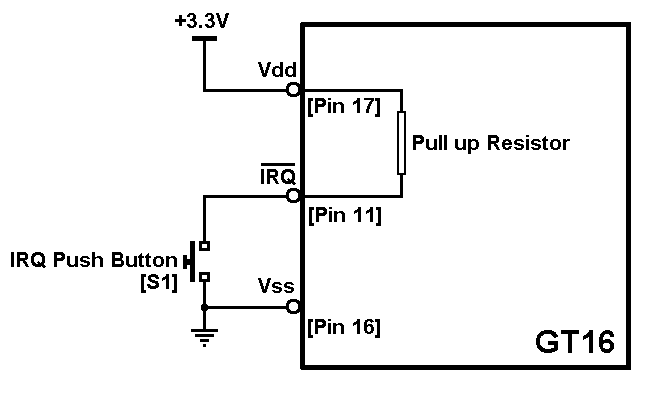
\includegraphics[width=0.7\textwidth]{model.png}
\caption{A block diagram illustrating the connections to the IRQ pin on the MCS08GT16A microcontroller (Please
note that your headings should be short descriptions of what is in the diagram not simply the figure title)}
\label{fig:model}
\end{figure}


\chapter{Methodology}

This is what I did to test and confirm my hypothesis.


You may want to split this chapter into sub chapters depending on your design. I suggest you change
the title to something more specific to your project.

This is where you describe your design process in detail, from component/device selection to actual
design implementation, to how you tested your system. Remember detail is important in technical
writing. Do not just write I used a computer give the computer specifications or the oscilloscopes part
number. Describe the system in enough detail so that someone else can replicate your design as well
as your testing methodology.

If you use or design code for your system, represent it as flow diagrams in text.

\chapter{Results}
These are the results I found from my investigation.

Present your results in a suitable format using tables and graphs where necessary. Remember to refer
to them in text and caption them properly.


\section{Simulation Results}


\section{Experimental Results}
\chapter{Discussion}

Here is what the results mean and how they tie to existing literature...

Discuss the relevance of your results and how they fit into the theoretical work you described in your
literature review.

\chapter{Conclusions}

These are the conclusions from the investivation and how the investigation changes things in this field or contributes to current knowledge...

Draw suitable and intelligent conclusions from your results and subsequent discussion.

\chapter{Recommendations}

Make sensible recommendations for further work.

Use the IEEE numbered reference style for referencing your work as shown in your thesis guidelines.
Please remember that the majority of your referenced work should be from journal articles, technical
reports and books not online sources such as Wikipedia.

\begin{thebibliography}{5}
\bibitem{smt2011} M. S. Tsoeu and M. Braae, ``Control Systems,'' \emph{IEEE}, {\bf vol. 34(3)}, pp. 123-129, 2011.
\bibitem{jct2010} J. C. Tapson, \emph{Instrumentation}, UCT Press, Cape Town, 2010.
\end{thebibliography}

\appendix
\chapter{Additional Files and Schematics}

Add any information here that you would like to have in your project but is not necessary in the main
text. Remember to refer to it in the main text. Separate your appendices based on what they are for
example. Equation derivations in Appendix A and code in Appendix B etc.

\chapter{Addenda}

\section{Ethics Forms}
}
\end{document}
